In addition to the numerical changes described in the previous section, a number of changes to the computational structure of the SE dynamical core were also made which both reduce the computational cost at both modest and large processor count.  In particular, new communication operators were developed which reduces the amount of data movement between MPI ranks as well as through the memory hierarchy. Derivative operators were optimized to increase code vectorization, and the limiter operator was rewritten to reduce cost.  A more detailed description of the optimizations can be found in \cite{dennis2017}.  

\begin{figure}[h]
\centering
 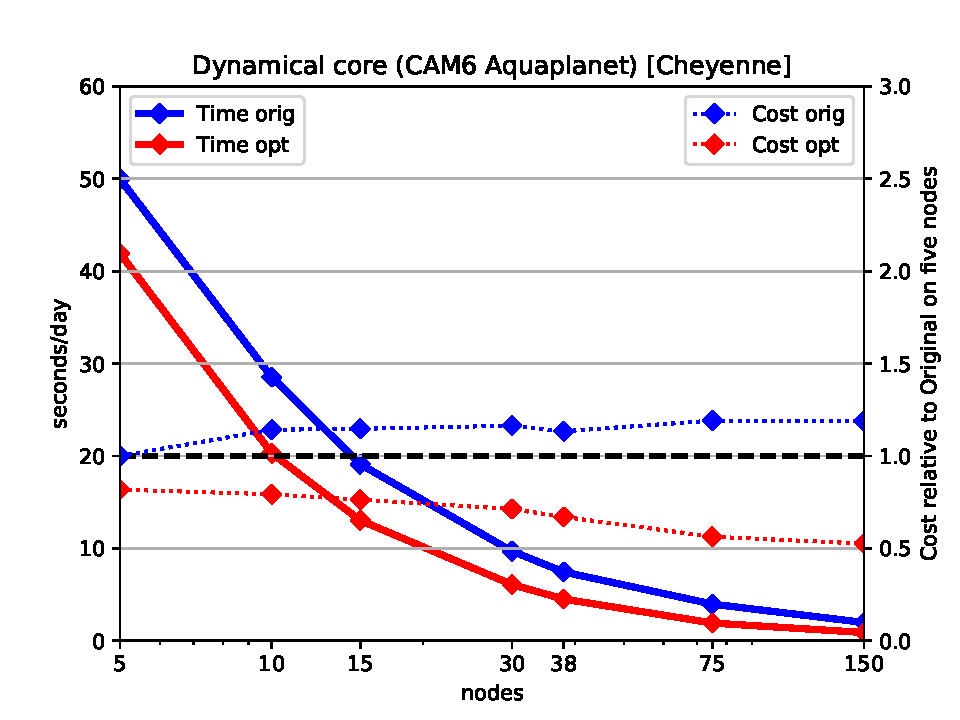
\includegraphics[scale=0.45]{figs/aqua-perf}
 \caption{The execution time of the SE dynamical core in an Aquaplanet configuration using CAM6 physics at NE=30 resolution on Cheyenne.   Both the original and optimized code is indicated by the solid blue and red lines, while the dotted lines represent the computational cost.}
 \label{fig:aqua-perf}
\end{figure}

We provide the execution time and computational cost for the dynamical core component of CAM in an Aquaplanet configuration for NE=30 resolution in Figure \ref{fig:aqua-perf} on Cheyenne. Cheyenne is an SGI ICE Cluster with 4,032 dual-socket Intel Xeon based nodes with 36 cores/node   The x-axis is the number of nodes while the left y-axis corresponds to execution time in seconds/day, and the right y-axis corresponds to the relative computational cost normalized to the original code run on five nodes or 180 cores of Cheyenne. Execution times and computational costs are also provided for up to 150 nodes or 5400 cores where a single spectral element is allocated to each core.

It is clear from Figure \ref{fig:aqua-perf} that the execution time for the dynamical core for the optimized version is significantly less than the original codebase for all core counts. The reduction in execution time for the optimized versus the original code varies from approximately 20\% at small core counts to slightly more than 50\% at larger core counts. The percentage reduction in execution time for the optimized versus original code is readily apparent by looking at the relative computational cost curves indicate by the dotted lines in Figure \ref{fig:aqua-perf}.  A value greater then run indicates that it is more expensive to run a particular configuration then the original code on five nodes, while a value less indicates that it is cheaper to run a particular configuration.  This approach allows for the comparison of both the impact of the optimizations have on a particular node code as well as the impact of optimizations to code scalability.  Interestingly while the original code becomes more expensive to execution at larger core counts the optimized code actually becomes cheaper to execute at larger core counts.  In particular, the greatest reduction of 40\% in computational cost occurs on 75 nodes.  We suspect that the decrease in computational cost illustrated in Figure \ref{fig:aqua-perf} is likely due to the fact that the calculations perform in the dynamical core now fit into the Level 3 (L3) cache on 75 nodes where they did not previously in either the original code base on the optimized code base on smaller node counts.  The decreased execution time due to the calculations being L3 cache resident is sufficiently large as to overcome any increase in execution time increase due to message passing.  

The relative cost of the dynamical core for the optimized code base is compared to other pieces of the Community Atmosphere Model is illustrated in Figure \ref{fig:percent}.  Note that for this comparison we use the same Aquaplanet CAM6 configuration, which achieves simulation rates that range from a low of 2.2 Simulated years per day (SYPD) on 5 nodes, to 53.4 SYPD on 150 nodes, and run for 1 month. This length of simulation includes the default monthly history I/O output as well as the generation of a restart file. We categorize four different pieces of CAM for timing purposes: physics, dynamics, I/O and the remapping of data-structures necessary between the physics and dynamics.  The faction of time that CAM spends performing the dynamics drops from a maximum of 41\% on five nodes, to a minimum of 22\% on 150 nodes.  While there is an increase in the relative cost for both the I/O and physics to dynamics interface, the largest relative increase in cost is seen in the physics calculations, that increase from 55\% of the time on five nodes to 66\% of the time on 150 nodes.  Figure \ref{fig:percent} illustrates that in CAM-SE the dynamical core is the most scalable component of the entire atmosphere model.  

\begin{figure}[h]
\centering
 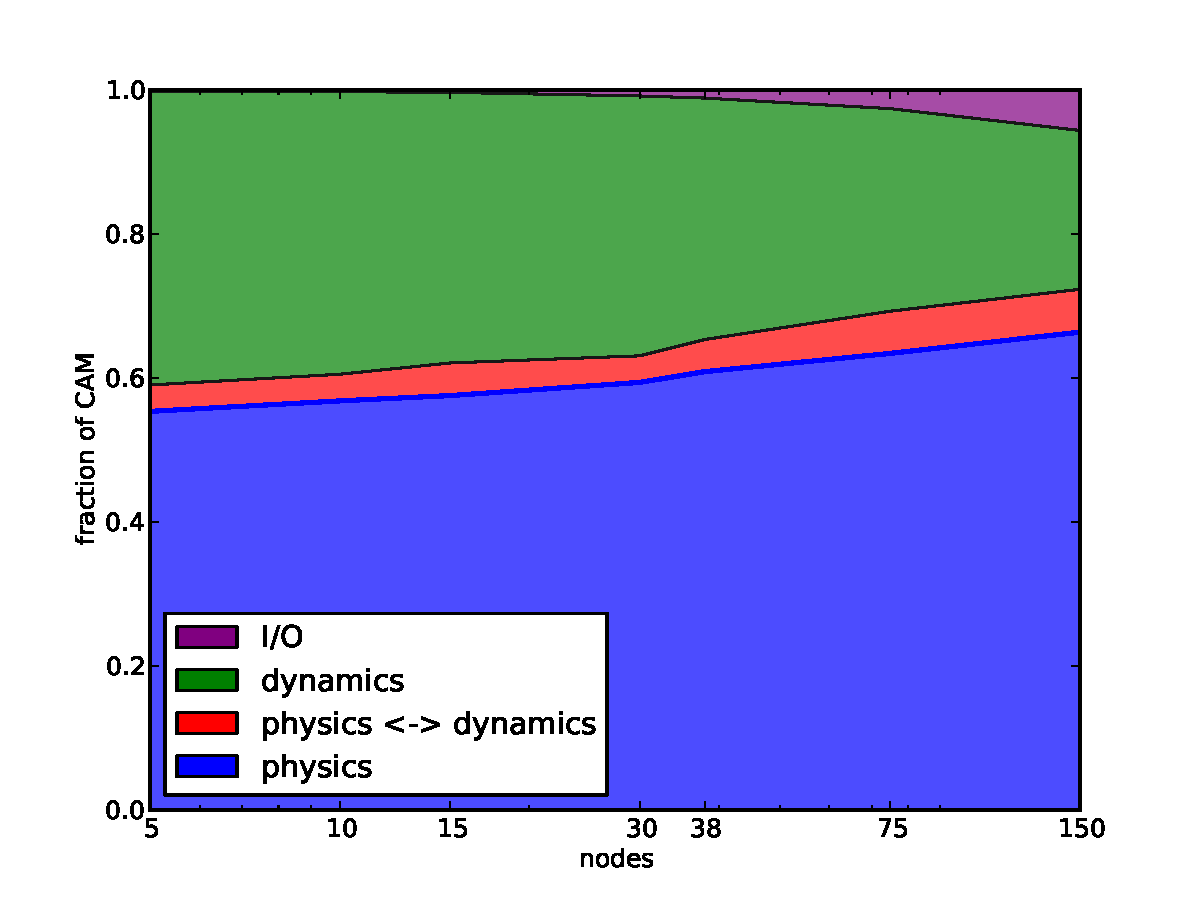
\includegraphics[scale=0.45]{figs/percent}
 \caption{Fraction of time spent in several different sub-components of CAM for NE=30 Aquaplanet simulation on Cheyenne.}
 \label{fig:percent}
\end{figure}

%       NEW
%   s:  2.24 SYPD
%   m:  4.18 SYPD
%   l:  6.82 SYPD
%  xl: 13.48 SYPD
% xxl: 16.66 SYPD
%  3x: 30.92 SYPD
%  4x: 53.36 SYPD

